\begin{appendices}

\chapter{Chaos analysis for oscilloscope quantization}\label{app: quantization}

The following plots represent the chaotic behavior of the system of four coupled blocks,
in which the oscilloscope quantization is progressively increased
(see Section~\ref{sec: oscilloscope quantization}).
For these analyses the driving voltage $V_d$ is always set to 0.05 V, and the number of points
in the sampled sequences is always $2\times 10^5$.
\begin{figure}[!htbp]
    \centering
    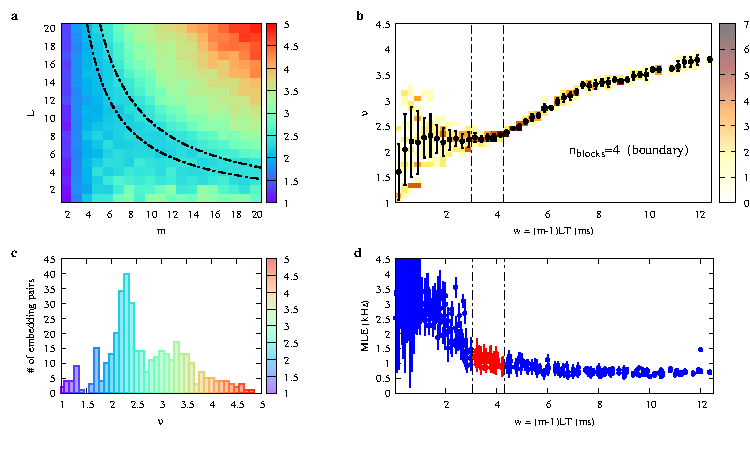
\includegraphics[width=\linewidth]{../blocks/4_blocks/2e5_points_new/plots/chaos_low.pdf}
    \caption{``Chasing chaos'' analysis of the experimental $W_1$ time series with 4 coupled blocks.
    (a) Map of estimated correlation dimension $\nu$ vs.\ embedding pair $(m, L)$.
    (b) Sample joint distribution of $(w,\nu)$ for the $\nu$-map in (a).
    (c) Histogram of the estimated $\nu$. (d) Distribution of MLE as a function of $w$.
    }\label{fig:4 blocks chaos}
\end{figure}

\begin{figure}[!htbp]
    \centering
    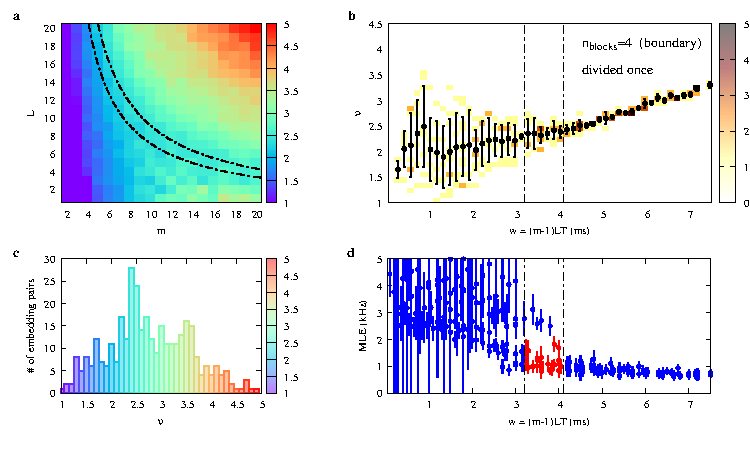
\includegraphics[width=\linewidth]{../blocks/4_blocks/2e5_points_new_divided/plots/chaos_low.pdf}
    \caption{``Chasing chaos'' analysis of the experimental $\tilde{W}_1$ time series with 4 coupled blocks.
    The oscilloscope quantization is doubled with respect to the case in Fig.~\ref{fig:4 blocks chaos}
    (a) Map of estimated correlation dimension $\nu$ vs.\ embedding pair $(m, L)$.
    (b) Sample joint distribution of $(w,\nu)$ for the $\nu$-map in (a).
    (c) Histogram of the estimated $\nu$. (d) Distribution of MLE as a function of $w$.
    }%A cluster of points, marked in red, can be identified in the uniformity region of (b), also highlighted here.}
    \label{fig:4 blocks chaos double quant}
\end{figure}

\begin{figure}[!htbp]
    \centering
    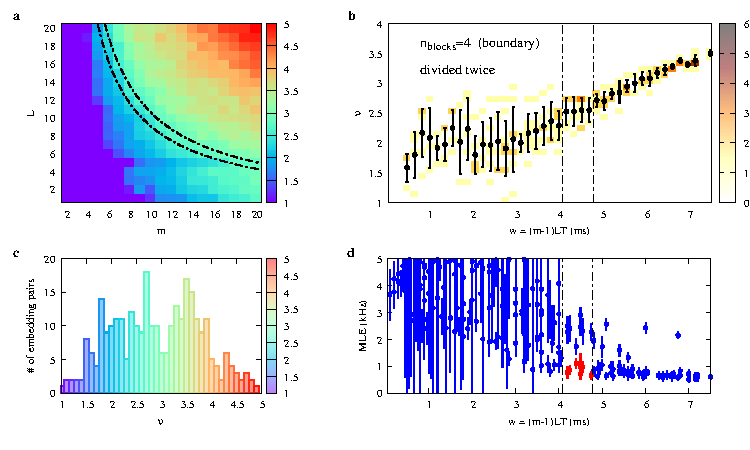
\includegraphics[width=\linewidth]{../blocks/4_blocks/2e5_points_new_divided_4/plots/chaos_low.pdf}
    \caption{``Chasing chaos'' analysis of the experimental $\tilde{\tilde{W}}_1$ time series with 4 coupled blocks.
    The oscilloscope quantization is quadrupled with respect to the case in Fig.~\ref{fig:4 blocks chaos}
    (a) Map of estimated correlation dimension $\nu$ vs.\ embedding pair $(m, L)$.
    (b) Sample joint distribution of $(w,\nu)$ for the $\nu$-map in (a).
    (c) Histogram of the estimated $\nu$. (d) Distribution of MLE as a function of $w$.
    }%A cluster of points, marked in red, can be identified in the uniformity region of (b), also highlighted here.}
    \label{fig:4 blocks chaos quadruple quant}
\end{figure}


\chapter{Chaos analysis on multiple coupled blocks}\label{app: multiple blocks}

The following plots represent the chaotic behavior of the system from 5 to 25 coupled blocks
(excluding 13 since it is presented in Section~\ref{sec: many blocks chaos}),
using the signal $W_1$ as the time series.
When the number of blocks is odd, an additional analysis was carried out on the signal $W_k$, where
the $k$-th block is located in the center (e.g.\ in the seven blocks case,
the analyzed signal will be $W_4$).
For these analyses the driving voltage $V_d$ is always set to 0.05 V, and the number of points
in the sampled sequences is always $2\times 10^5$.

\begin{figure}[!htbp]
    \centering
    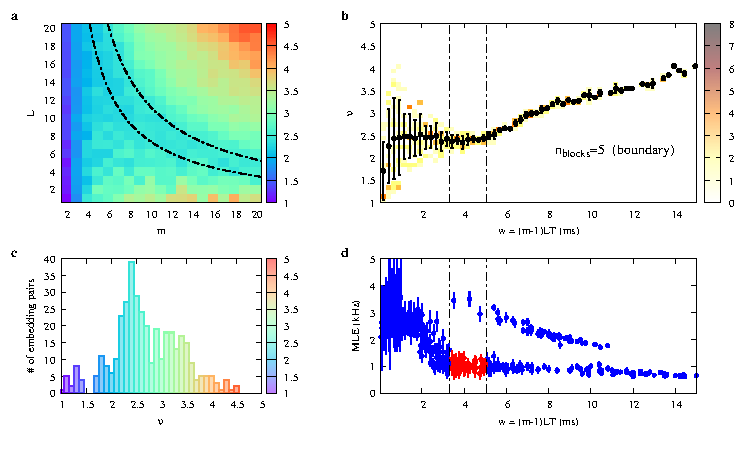
\includegraphics[width=\linewidth]{../blocks/5_blocks/edge/2e5_points/plots/chaos_low.pdf}
    \caption{``Chasing chaos'' analysis of the experimental $W_1$ time series with 5 coupled blocks.
    (a) Map of estimated correlation dimension $\nu$ vs.\ embedding pair $(m, L)$.
    (b) Sample joint distribution of $(w,\nu)$ for the $\nu$-map in (a).
    (c) Histogram of the estimated $\nu$. (d) Distribution of MLE as a function of $w$.
    } 
\end{figure}

\begin{figure}[!htbp]
    \centering
    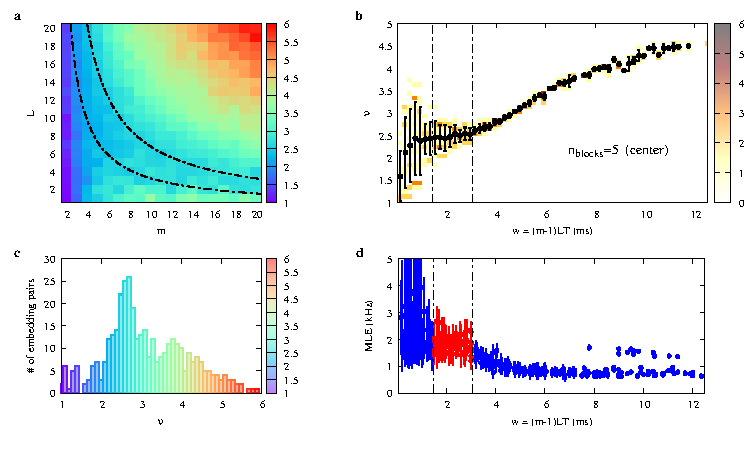
\includegraphics[width=\linewidth]{../blocks/5_blocks/middle/2e5_points/plots/chaos_low.pdf}
    \caption{``Chasing chaos'' analysis of the experimental $W_3$ time series with 5 coupled blocks.
    (a) Map of estimated correlation dimension $\nu$ vs.\ embedding pair $(m, L)$.
    (b) Sample joint distribution of $(w,\nu)$ for the $\nu$-map in (a).
    (c) Histogram of the estimated $\nu$. (d) Distribution of MLE as a function of $w$.
    } 
\end{figure}

\begin{figure}[!htbp]
    \centering
    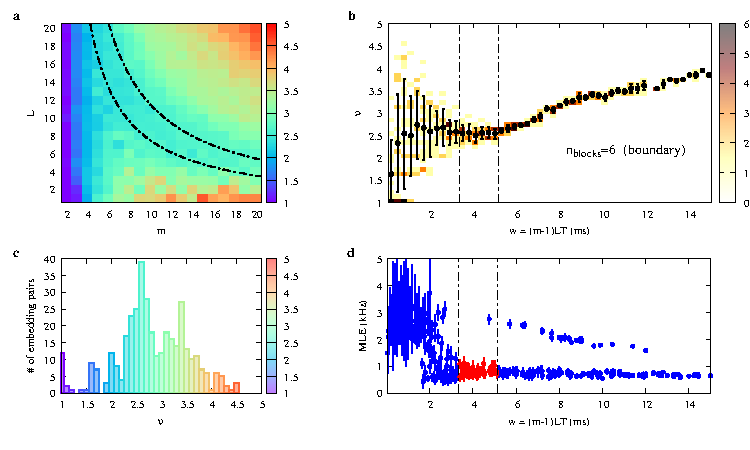
\includegraphics[width=\linewidth]{../blocks/6_blocks/2e5_points/plots/chaos_low.pdf}
    \caption{``Chasing chaos'' analysis of the experimental $W_1$ time series with 6 coupled blocks.
    (a) Map of estimated correlation dimension $\nu$ vs.\ embedding pair $(m, L)$.
    (b) Sample joint distribution of $(w,\nu)$ for the $\nu$-map in (a).
    (c) Histogram of the estimated $\nu$. (d) Distribution of MLE as a function of $w$.
    } 
\end{figure}

\begin{figure}[!htbp]
    \centering
    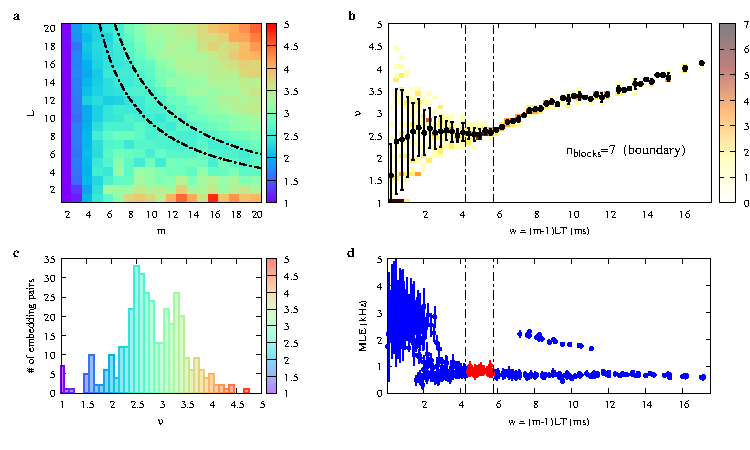
\includegraphics[width=\linewidth]{../blocks/7_blocks/edge/2e5_points/plots/chaos_low.pdf}
    \caption{``Chasing chaos'' analysis of the experimental $W_1$ time series with 7 coupled blocks.
    (a) Map of estimated correlation dimension $\nu$ vs.\ embedding pair $(m, L)$.
    (b) Sample joint distribution of $(w,\nu)$ for the $\nu$-map in (a).
    (c) Histogram of the estimated $\nu$. (d) Distribution of MLE as a function of $w$.
    } 
\end{figure}

\begin{figure}[!htbp]
    \centering
    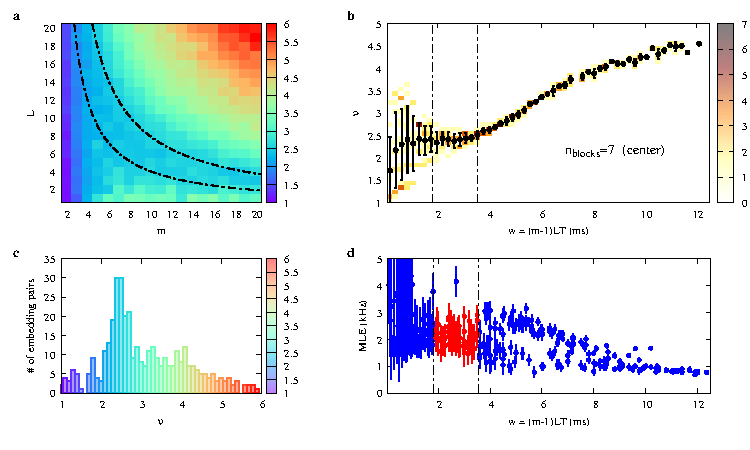
\includegraphics[width=\linewidth]{../blocks/7_blocks/middle/2e5_points/plots/chaos_low.pdf}
    \caption{``Chasing chaos'' analysis of the experimental $W_4$ time series with 7 coupled blocks.
    (a) Map of estimated correlation dimension $\nu$ vs.\ embedding pair $(m, L)$.
    (b) Sample joint distribution of $(w,\nu)$ for the $\nu$-map in (a).
    (c) Histogram of the estimated $\nu$. (d) Distribution of MLE as a function of $w$.
    } 
\end{figure}

\begin{figure}[!htbp]
    \centering
    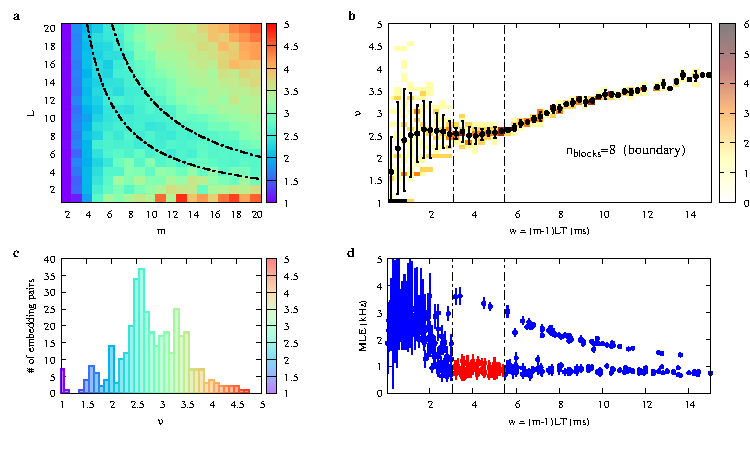
\includegraphics[width=\linewidth]{../blocks/8_blocks/2e5_points/plots/chaos_low.pdf}
    \caption{``Chasing chaos'' analysis of the experimental $W_1$ time series with 8 coupled blocks.
    (a) Map of estimated correlation dimension $\nu$ vs.\ embedding pair $(m, L)$.
    (b) Sample joint distribution of $(w,\nu)$ for the $\nu$-map in (a).
    (c) Histogram of the estimated $\nu$. (d) Distribution of MLE as a function of $w$.
    } 
\end{figure}

\begin{figure}[!htbp]
    \centering
    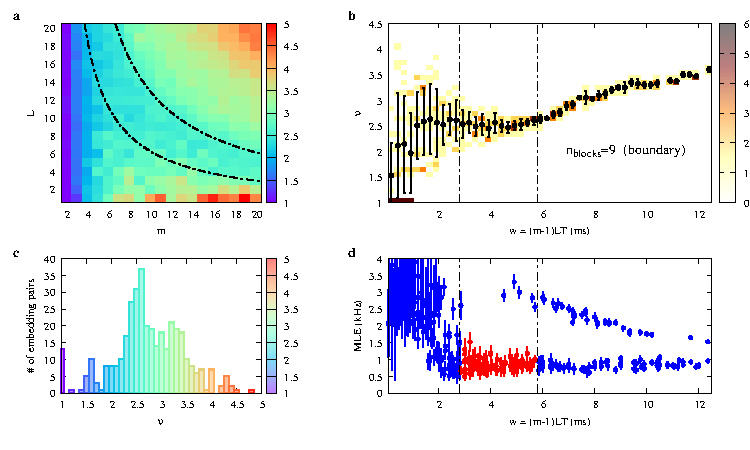
\includegraphics[width=\linewidth]{../blocks/9_blocks/edge/2e5_points/plots/chaos_low.pdf}
    \caption{``Chasing chaos'' analysis of the experimental $W_1$ time series with 9 coupled blocks.
    (a) Map of estimated correlation dimension $\nu$ vs.\ embedding pair $(m, L)$.
    (b) Sample joint distribution of $(w,\nu)$ for the $\nu$-map in (a).
    (c) Histogram of the estimated $\nu$. (d) Distribution of MLE as a function of $w$.
    } 
\end{figure}

\begin{figure}[!htbp]
    \centering
    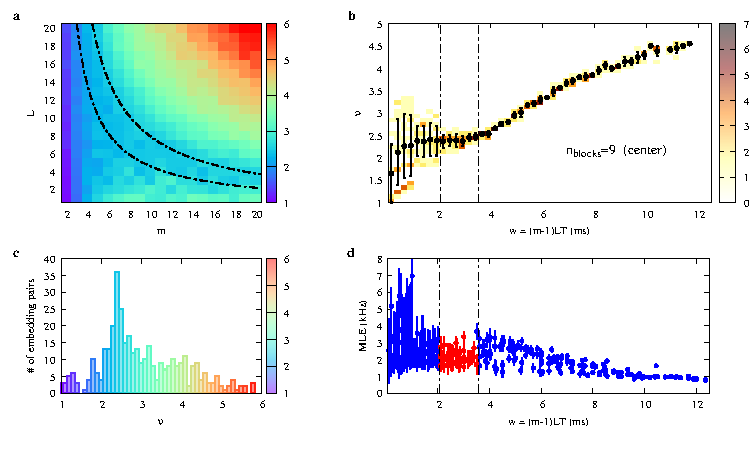
\includegraphics[width=\linewidth]{../blocks/9_blocks/middle/2e5_points/plots/chaos_low.pdf}
    \caption{``Chasing chaos'' analysis of the experimental $W_5$ time series with 9 coupled blocks.
    (a) Map of estimated correlation dimension $\nu$ vs.\ embedding pair $(m, L)$.
    (b) Sample joint distribution of $(w,\nu)$ for the $\nu$-map in (a).
    (c) Histogram of the estimated $\nu$. (d) Distribution of MLE as a function of $w$.
    } 
\end{figure}

\begin{figure}[!htbp]
    \centering
    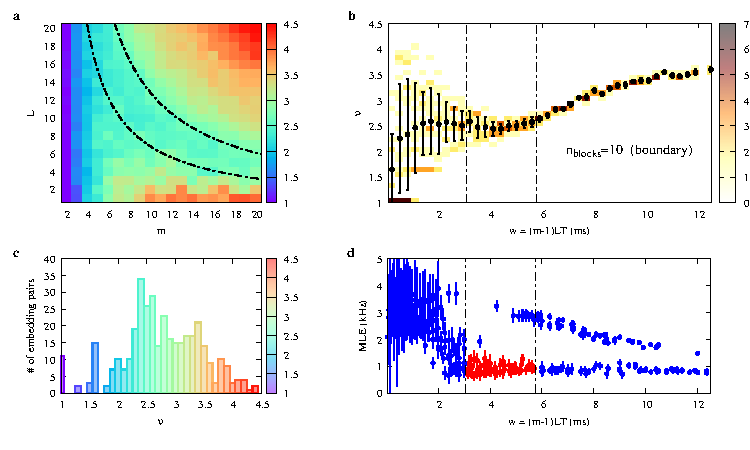
\includegraphics[width=\linewidth]{../blocks/10_blocks/2e5_points/plots/chaos_low.pdf}
    \caption{``Chasing chaos'' analysis of the experimental $W_1$ time series with 10 coupled blocks.
    (a) Map of estimated correlation dimension $\nu$ vs.\ embedding pair $(m, L)$.
    (b) Sample joint distribution of $(w,\nu)$ for the $\nu$-map in (a).
    (c) Histogram of the estimated $\nu$. (d) Distribution of MLE as a function of $w$.
    } 
\end{figure}

\begin{figure}[!htbp]
    \centering
    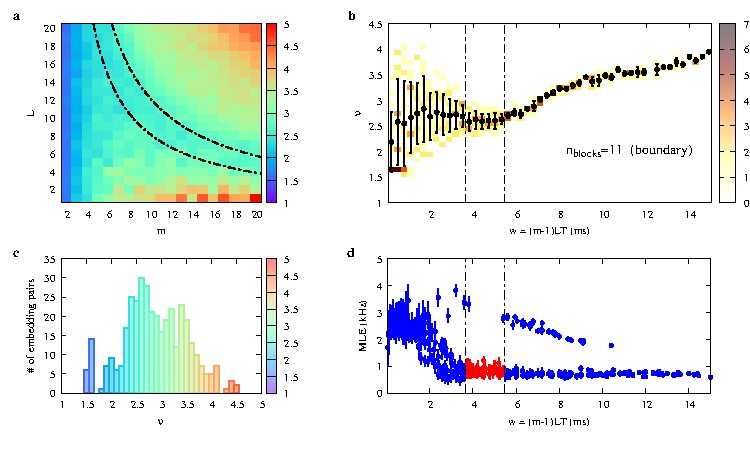
\includegraphics[width=\linewidth]{../blocks/11_blocks/edge/2e5_points/plots/chaos_low.pdf}
    \caption{``Chasing chaos'' analysis of the experimental $W_1$ time series with 11 coupled blocks.
    (a) Map of estimated correlation dimension $\nu$ vs.\ embedding pair $(m, L)$.
    (b) Sample joint distribution of $(w,\nu)$ for the $\nu$-map in (a).
    (c) Histogram of the estimated $\nu$. (d) Distribution of MLE as a function of $w$.
    } 
\end{figure}

\begin{figure}[!htbp]
    \centering
    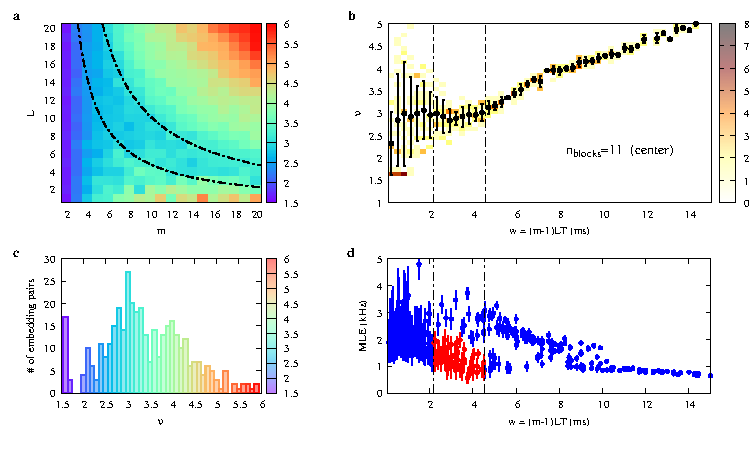
\includegraphics[width=\linewidth]{../blocks/11_blocks/middle/2e5_points/plots/chaos_low.pdf}
    \caption{``Chasing chaos'' analysis of the experimental $W_6$ time series with 11 coupled blocks.
    (a) Map of estimated correlation dimension $\nu$ vs.\ embedding pair $(m, L)$.
    (b) Sample joint distribution of $(w,\nu)$ for the $\nu$-map in (a).
    (c) Histogram of the estimated $\nu$. (d) Distribution of MLE as a function of $w$.
    } 
\end{figure}

\begin{figure}[!htbp]
    \centering
    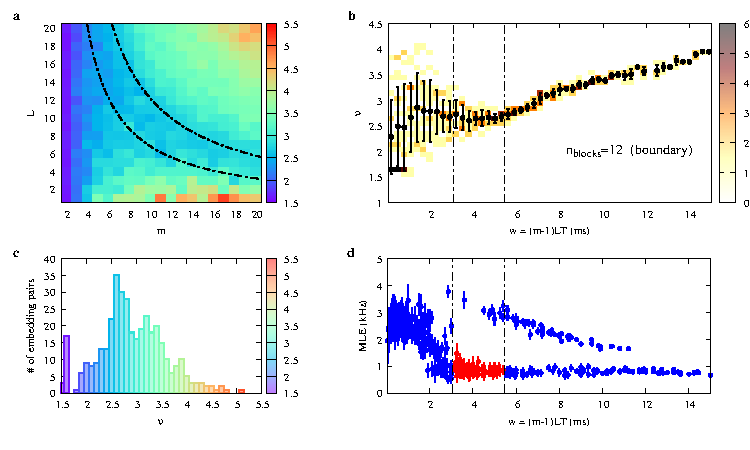
\includegraphics[width=\linewidth]{../blocks/12_blocks/2e5_points/plots/chaos_low.pdf}
    \caption{``Chasing chaos'' analysis of the experimental $W_1$ time series with 12 coupled blocks.
    (a) Map of estimated correlation dimension $\nu$ vs.\ embedding pair $(m, L)$.
    (b) Sample joint distribution of $(w,\nu)$ for the $\nu$-map in (a).
    (c) Histogram of the estimated $\nu$. (d) Distribution of MLE as a function of $w$.
    } 
\end{figure}

\begin{figure}[!htbp]
    \centering
    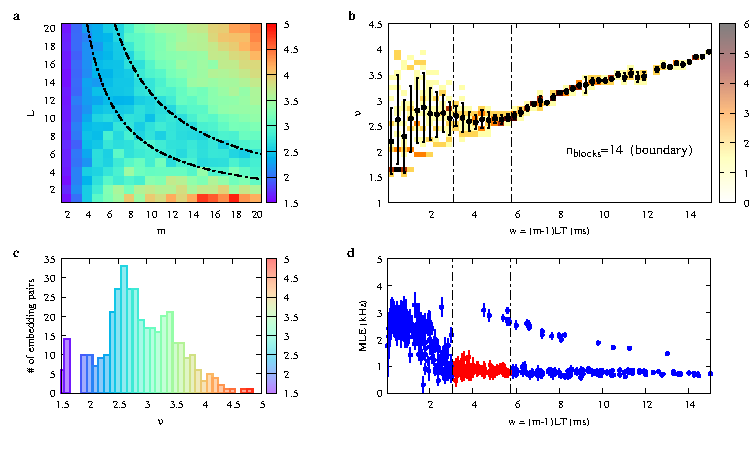
\includegraphics[width=\linewidth]{../blocks/14_blocks/2e5_points/plots/chaos_low.pdf}
    \caption{``Chasing chaos'' analysis of the experimental $W_1$ time series with 14 coupled blocks.
    (a) Map of estimated correlation dimension $\nu$ vs.\ embedding pair $(m, L)$.
    (b) Sample joint distribution of $(w,\nu)$ for the $\nu$-map in (a).
    (c) Histogram of the estimated $\nu$. (d) Distribution of MLE as a function of $w$.
    } 
\end{figure}

\begin{figure}[!htbp]
    \centering
    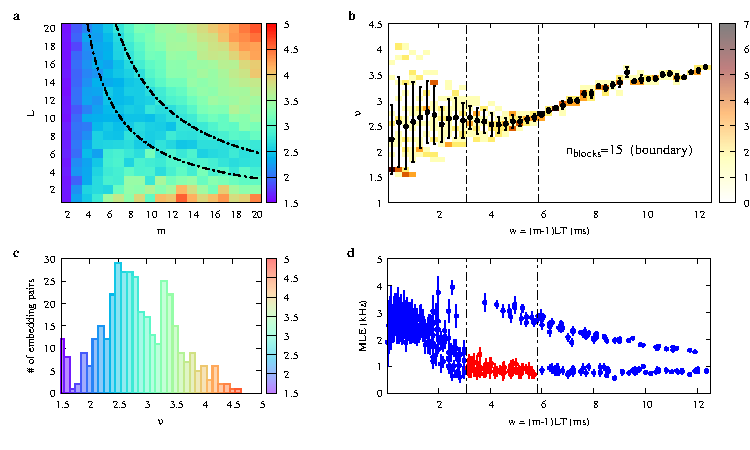
\includegraphics[width=\linewidth]{../blocks/15_blocks/edge/2e5_points/plots/chaos_low.pdf}
    \caption{``Chasing chaos'' analysis of the experimental $W_1$ time series with 15 coupled blocks.
    (a) Map of estimated correlation dimension $\nu$ vs.\ embedding pair $(m, L)$.
    (b) Sample joint distribution of $(w,\nu)$ for the $\nu$-map in (a).
    (c) Histogram of the estimated $\nu$. (d) Distribution of MLE as a function of $w$.
    } 
\end{figure}

\begin{figure}[!htbp]
    \centering
    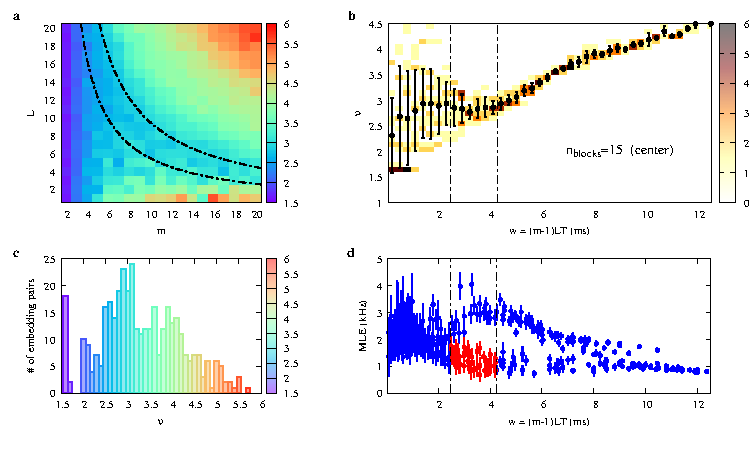
\includegraphics[width=\linewidth]{../blocks/15_blocks/middle/2e5_points/plots/chaos_low.pdf}
    \caption{``Chasing chaos'' analysis of the experimental $W_8$ time series with 15 coupled blocks.
    (a) Map of estimated correlation dimension $\nu$ vs.\ embedding pair $(m, L)$.
    (b) Sample joint distribution of $(w,\nu)$ for the $\nu$-map in (a).
    (c) Histogram of the estimated $\nu$. (d) Distribution of MLE as a function of $w$.
    } 
\end{figure}

\begin{figure}[!htbp]
    \centering
    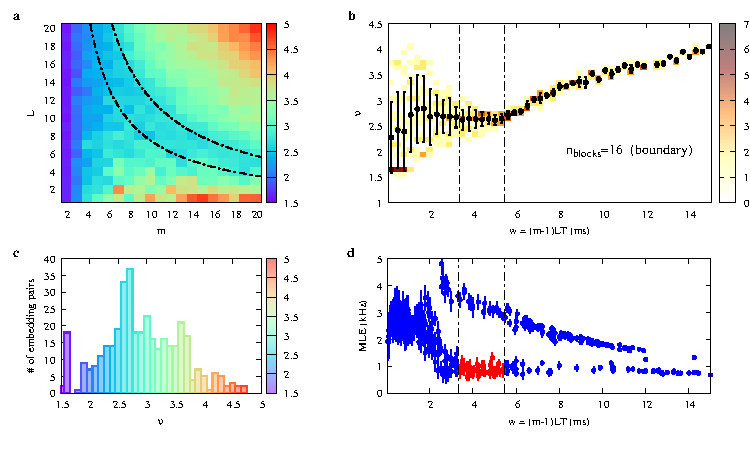
\includegraphics[width=\linewidth]{../blocks/16_blocks/2e5_points/plots/chaos_low.pdf}
    \caption{``Chasing chaos'' analysis of the experimental $W_1$ time series with 16 coupled blocks.
    (a) Map of estimated correlation dimension $\nu$ vs.\ embedding pair $(m, L)$.
    (b) Sample joint distribution of $(w,\nu)$ for the $\nu$-map in (a).
    (c) Histogram of the estimated $\nu$. (d) Distribution of MLE as a function of $w$.
    } 
\end{figure}

\begin{figure}[!htbp]
    \centering
    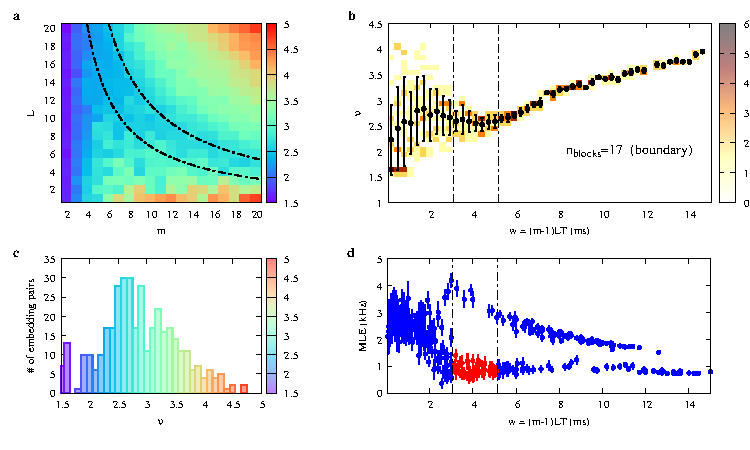
\includegraphics[width=\linewidth]{../blocks/17_blocks/edge/2e5_points/plots/chaos_low.pdf}
    \caption{``Chasing chaos'' analysis of the experimental $W_1$ time series with 17 coupled blocks.
    (a) Map of estimated correlation dimension $\nu$ vs.\ embedding pair $(m, L)$.
    (b) Sample joint distribution of $(w,\nu)$ for the $\nu$-map in (a).
    (c) Histogram of the estimated $\nu$. (d) Distribution of MLE as a function of $w$.
    } 
\end{figure}

\begin{figure}[!htbp]
    \centering
    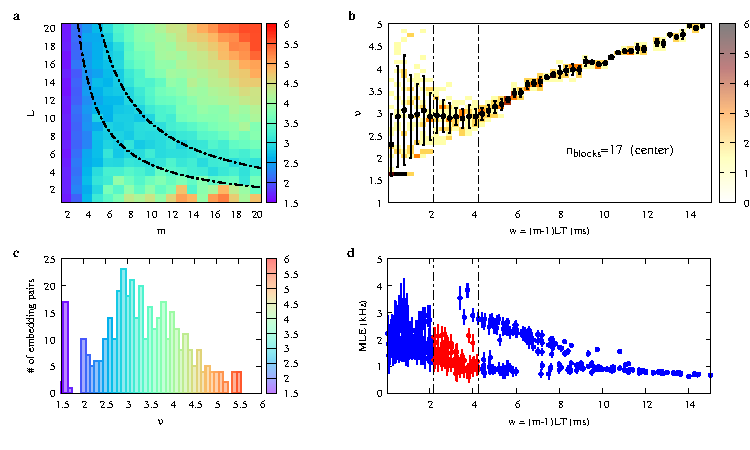
\includegraphics[width=\linewidth]{../blocks/17_blocks/middle/2e5_points/plots/chaos_low.pdf}
    \caption{``Chasing chaos'' analysis of the experimental $W_9$ time series with 17 coupled blocks.
    (a) Map of estimated correlation dimension $\nu$ vs.\ embedding pair $(m, L)$.
    (b) Sample joint distribution of $(w,\nu)$ for the $\nu$-map in (a).
    (c) Histogram of the estimated $\nu$. (d) Distribution of MLE as a function of $w$.
    } 
\end{figure}

\begin{figure}[!htbp]
    \centering
    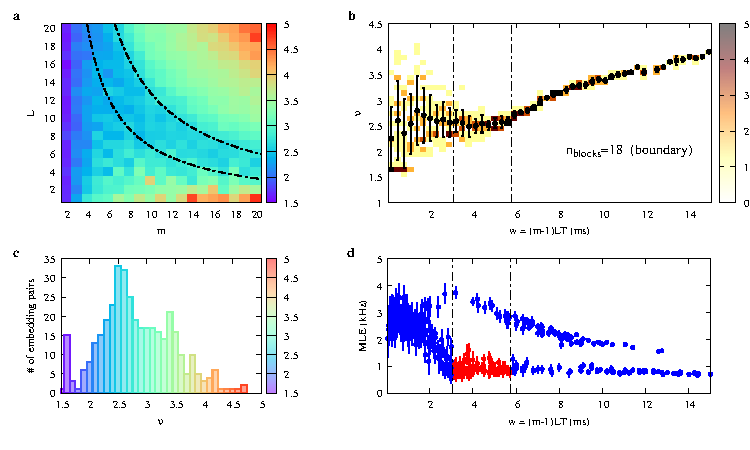
\includegraphics[width=\linewidth]{../blocks/18_blocks/2e5_points/plots/chaos_low.pdf}
    \caption{``Chasing chaos'' analysis of the experimental $W_1$ time series with 18 coupled blocks.
    (a) Map of estimated correlation dimension $\nu$ vs.\ embedding pair $(m, L)$.
    (b) Sample joint distribution of $(w,\nu)$ for the $\nu$-map in (a).
    (c) Histogram of the estimated $\nu$. (d) Distribution of MLE as a function of $w$.
    } 
\end{figure}

\begin{figure}[!htbp]
    \centering
    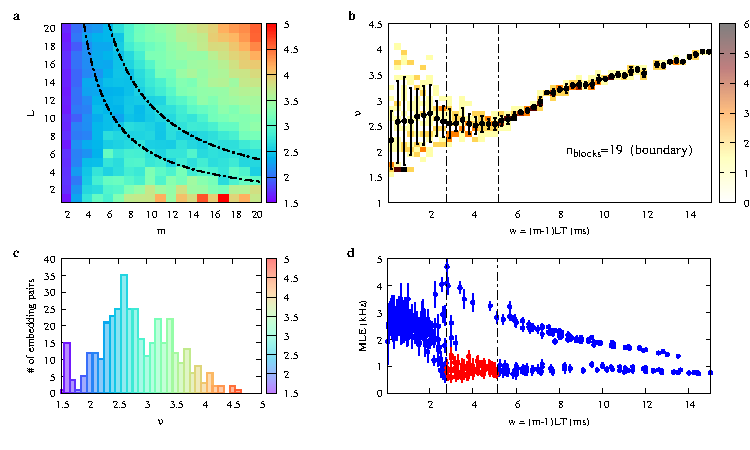
\includegraphics[width=\linewidth]{../blocks/19_blocks/edge/2e5_points/plots/chaos_low.pdf}
    \caption{``Chasing chaos'' analysis of the experimental $W_1$ time series with 19 coupled blocks.
    (a) Map of estimated correlation dimension $\nu$ vs.\ embedding pair $(m, L)$.
    (b) Sample joint distribution of $(w,\nu)$ for the $\nu$-map in (a).
    (c) Histogram of the estimated $\nu$. (d) Distribution of MLE as a function of $w$.
    } 
\end{figure}

\begin{figure}[!htbp]
    \centering
    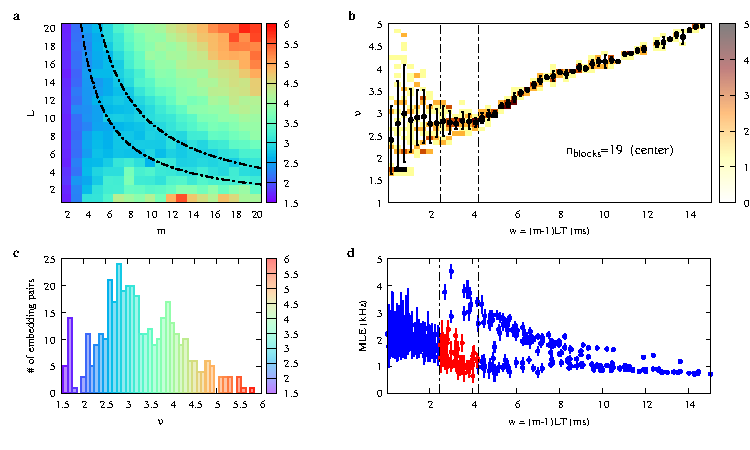
\includegraphics[width=\linewidth]{../blocks/19_blocks/middle/2e5_points/plots/chaos_low.pdf}
    \caption{``Chasing chaos'' analysis of the experimental $W_{10}$ time series with 19 coupled blocks.
    (a) Map of estimated correlation dimension $\nu$ vs.\ embedding pair $(m, L)$.
    (b) Sample joint distribution of $(w,\nu)$ for the $\nu$-map in (a).
    (c) Histogram of the estimated $\nu$. (d) Distribution of MLE as a function of $w$.
    } 
\end{figure}

\begin{figure}[!htbp]
    \centering
    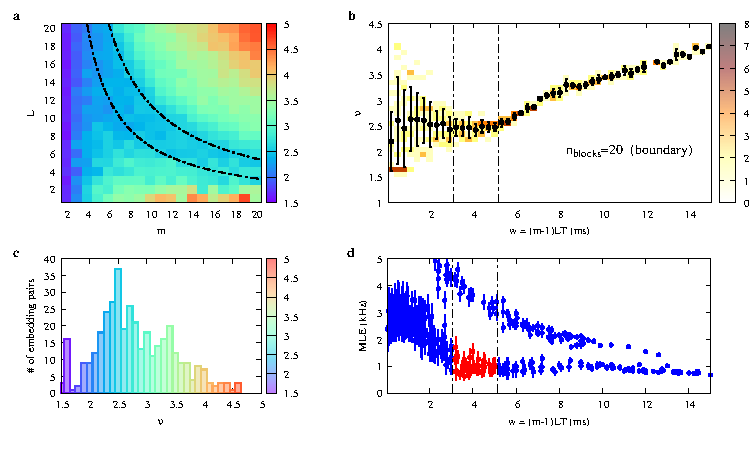
\includegraphics[width=\linewidth]{../blocks/20_blocks/2e5_points/plots/chaos_low.pdf}
    \caption{``Chasing chaos'' analysis of the experimental $W_1$ time series with 20 coupled blocks.
    (a) Map of estimated correlation dimension $\nu$ vs.\ embedding pair $(m, L)$.
    (b) Sample joint distribution of $(w,\nu)$ for the $\nu$-map in (a).
    (c) Histogram of the estimated $\nu$. (d) Distribution of MLE as a function of $w$.
    } 
\end{figure}

\begin{figure}[!htbp]
    \centering
    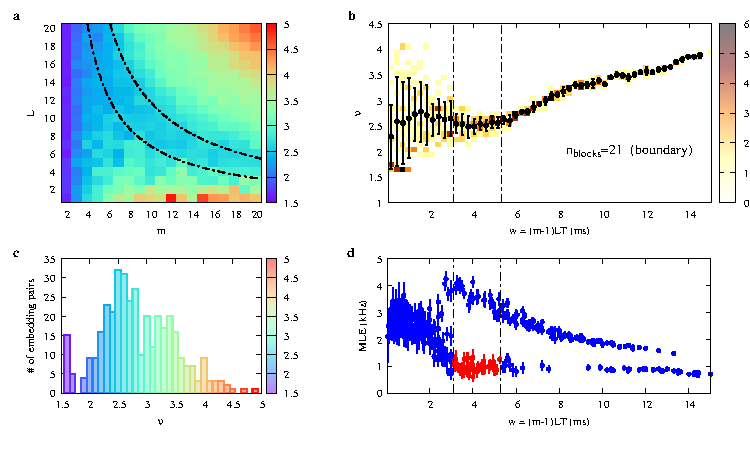
\includegraphics[width=\linewidth]{../blocks/21_blocks/edge/2e5_points/plots/chaos_low.pdf}
    \caption{``Chasing chaos'' analysis of the experimental $W_1$ time series with 21 coupled blocks.
    (a) Map of estimated correlation dimension $\nu$ vs.\ embedding pair $(m, L)$.
    (b) Sample joint distribution of $(w,\nu)$ for the $\nu$-map in (a).
    (c) Histogram of the estimated $\nu$. (d) Distribution of MLE as a function of $w$.
    } 
\end{figure}

\begin{figure}[!htbp]
    \centering
    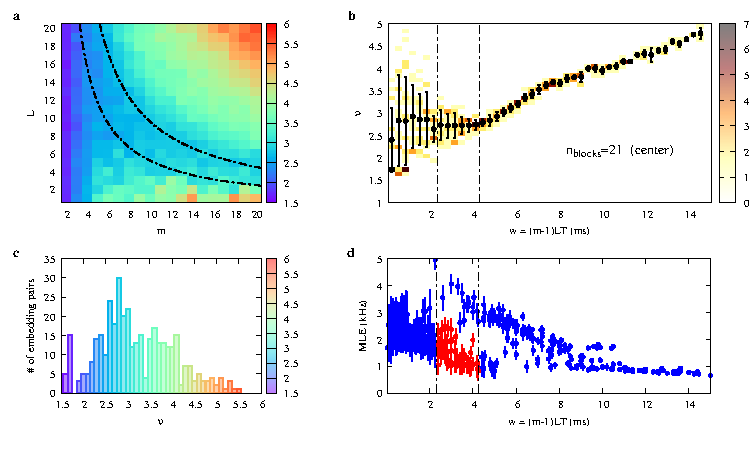
\includegraphics[width=\linewidth]{../blocks/21_blocks/middle/2e5_points/plots/chaos_low.pdf}
    \caption{``Chasing chaos'' analysis of the experimental $W_{11}$ time series with 21 coupled blocks.
    (a) Map of estimated correlation dimension $\nu$ vs.\ embedding pair $(m, L)$.
    (b) Sample joint distribution of $(w,\nu)$ for the $\nu$-map in (a).
    (c) Histogram of the estimated $\nu$. (d) Distribution of MLE as a function of $w$.
    } 
\end{figure}

\begin{figure}[!htbp]
    \centering
    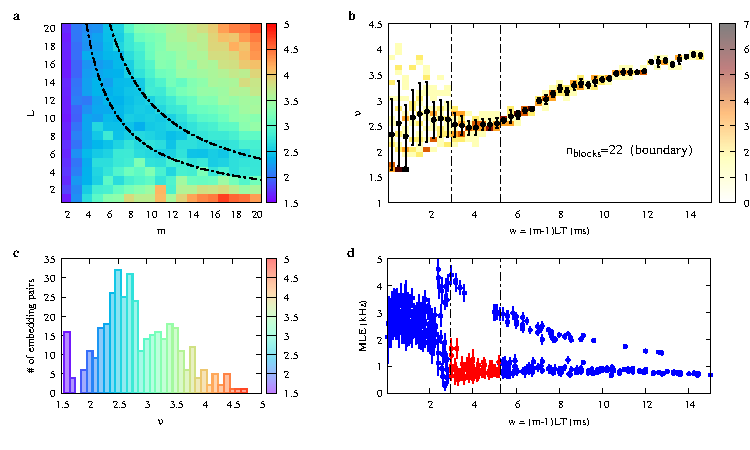
\includegraphics[width=\linewidth]{../blocks/22_blocks/2e5_points/plots/chaos_low.pdf}
    \caption{``Chasing chaos'' analysis of the experimental $W_1$ time series with 22 coupled blocks.
    (a) Map of estimated correlation dimension $\nu$ vs.\ embedding pair $(m, L)$.
    (b) Sample joint distribution of $(w,\nu)$ for the $\nu$-map in (a).
    (c) Histogram of the estimated $\nu$. (d) Distribution of MLE as a function of $w$.
    } 
\end{figure}

\begin{figure}[!htbp]
    \centering
    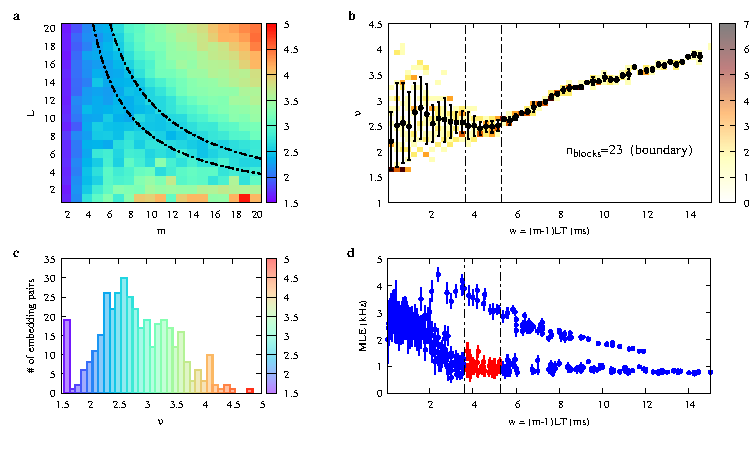
\includegraphics[width=\linewidth]{../blocks/23_blocks/edge/2e5_points/plots/chaos_low.pdf}
    \caption{``Chasing chaos'' analysis of the experimental $W_1$ time series with 23 coupled blocks.
    (a) Map of estimated correlation dimension $\nu$ vs.\ embedding pair $(m, L)$.
    (b) Sample joint distribution of $(w,\nu)$ for the $\nu$-map in (a).
    (c) Histogram of the estimated $\nu$. (d) Distribution of MLE as a function of $w$.
    } 
\end{figure}

\begin{figure}[!htbp]
    \centering
    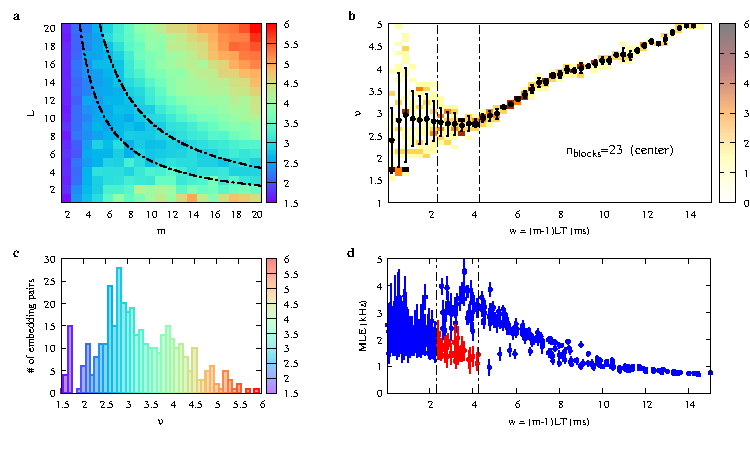
\includegraphics[width=\linewidth]{../blocks/23_blocks/middle/2e5_points/plots/chaos_low.pdf}
    \caption{``Chasing chaos'' analysis of the experimental $W_{12}$ time series with 23 coupled blocks.
    (a) Map of estimated correlation dimension $\nu$ vs.\ embedding pair $(m, L)$.
    (b) Sample joint distribution of $(w,\nu)$ for the $\nu$-map in (a).
    (c) Histogram of the estimated $\nu$. (d) Distribution of MLE as a function of $w$.
    } 
\end{figure}

\begin{figure}[!htbp]
    \centering
    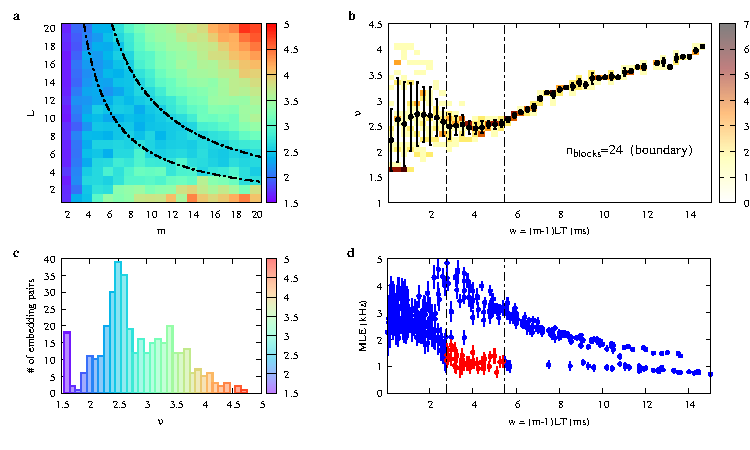
\includegraphics[width=\linewidth]{../blocks/24_blocks/2e5_points/plots/chaos_low.pdf}
    \caption{``Chasing chaos'' analysis of the experimental $W_1$ time series with 24 coupled blocks.
    (a) Map of estimated correlation dimension $\nu$ vs.\ embedding pair $(m, L)$.
    (b) Sample joint distribution of $(w,\nu)$ for the $\nu$-map in (a).
    (c) Histogram of the estimated $\nu$. (d) Distribution of MLE as a function of $w$.
    } 
\end{figure}

\begin{figure}[!htbp]
    \centering
    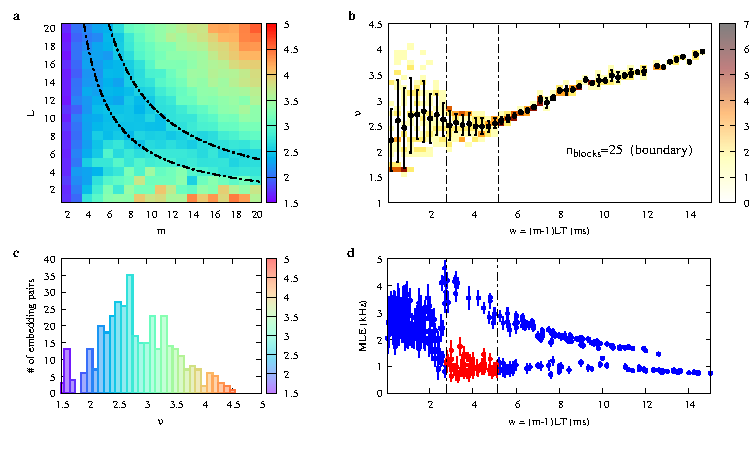
\includegraphics[width=\linewidth]{../blocks/25_blocks/edge/2e5_points/plots/chaos_low.pdf}
    \caption{``Chasing chaos'' analysis of the experimental $W_1$ time series with 25 coupled blocks.
    (a) Map of estimated correlation dimension $\nu$ vs.\ embedding pair $(m, L)$.
    (b) Sample joint distribution of $(w,\nu)$ for the $\nu$-map in (a).
    (c) Histogram of the estimated $\nu$. (d) Distribution of MLE as a function of $w$.
    } 
\end{figure}

\begin{figure}[!htbp]
    \centering
    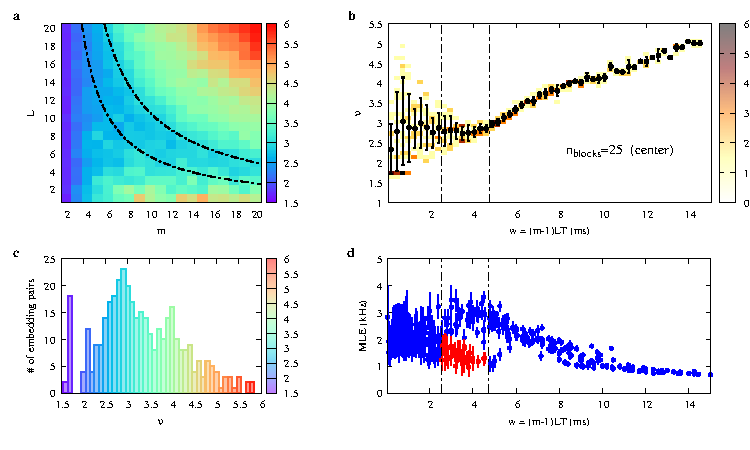
\includegraphics[width=\linewidth]{../blocks/25_blocks/middle/2e5_points/plots/chaos_low.pdf}
    \caption{``Chasing chaos'' analysis of the experimental $W_{13}$ time series with 25 coupled blocks.
    (a) Map of estimated correlation dimension $\nu$ vs.\ embedding pair $(m, L)$.
    (b) Sample joint distribution of $(w,\nu)$ for the $\nu$-map in (a).
    (c) Histogram of the estimated $\nu$. (d) Distribution of MLE as a function of $w$.
    } 
\end{figure}








\end{appendices}